
\chapter{Examples}\label{chap2}
WE\pageoriginale NOW DESCRIBE some problems which lead to the non-linear equation
$$
\phi_t+c(\phi)\phi_x=0.
$$

In most of the problems we relate two quantities: $\rho(x,t)$ which is the density of something per unit length and $q(x,t)$ which is the flow per unit time. If the `something' is conserved, then for a section $x_2\leq x\leq x_1$ we have the conservation equation 
\begin{equation}
\frac{d}{dt}\int\limits_{x_2}^{x_1}\rho\,dx+q(x_1,t)-q(x_2,t) =0.\label{chap2:eq2.1}
\end{equation}

\begin{figure}[H]
\centering
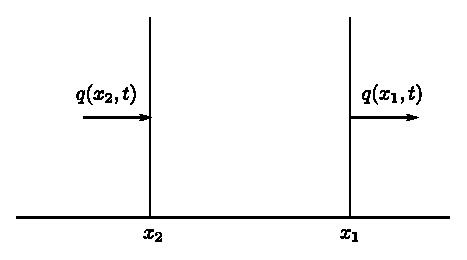
\includegraphics{figures/fig61-2.1.eps}
\caption{}
\label{chap1:fig2.1}
\end{figure}


If $\rho$ and $q$ are continuously differentiable then in the limit $x_1\to x_2$, equation \eqref{chap2:eq2.1} becomes
\begin{equation}
\frac{\partial\rho}{\partial t}+\frac{\partial q}{\partial x} =0.\label{chap2:eq2.2}
\end{equation}

If there exists also a functional relation $\rho =Q(\rho)$ (this is so to a first approximation in many cases) then \eqref{chap2:eq2.2} can be written as
\begin{equation}
\rho_t+c(\rho)\rho_x=0,\label{chap2:eq2.3}
\end{equation}\pageoriginale
where $c(\rho)=Q'(\rho)$.

We will now give some specific examples.

\section{Traffic Flow}\label{chap2:sec2.1}

We consider the flow of cars on a long highway. Here $\rho$ will be the number of cars per unit length. Let $v$ be the average local velocity of the cars. Then $q$, the flow per unit time, is given by $q=\rho v$. For a long section of highway with no exits or entrances the cars are conserved so that \eqref{chap2:eq2.1} holds. It also seems reasonable to assume that on the average $v$ is a function of $\rho$ to a first approximation. Hence $\rho$ satisfies \eqref{chap2:eq2.3}. The velocity $v$ will be a decreasing function $V(\rho)$, and $Q(\rho)=\rho V(\rho)$. When the density is small the velocity will be some upper limiting value, and when the density is maximum the velocity will be zero. Therefore the graph of $V$ will take a form as shown in the figure 2.2.

\begin{figure}[H]
\centering
\includegraphics[scale=.9]{figures/fig61-2.2.eps}
\caption{}
\label{chap1:fig2.2}
\end{figure}

Since $q=Q(\rho)=\rho V$, there will be no flow when the velocity is maximum (\ie $\rho =0$) and when $\rho$ is maximum (\ie $V=0$). Hence\pageoriginale the graph of $Q(\rho)$ will look like the figure 2.3.

It was found in one set of observations on U.S. highways that the maximum density is approximately 225 vehicles per mile (per traffic lane), and the maximum flow is approximately 1500 vehicles per hour. When the flow $q$ is maximum the density is found to be around 80 vehicles per mile.

\begin{figure}[H]
\centering
\includegraphics{figures/fig61-2.3.eps}
\caption{}
\label{chap1:fig2.3}
\end{figure}

The propagation speed for the wave is $c(\rho)=Q'(\rho)=V(\rho)+\frac{dV}{d\rho}$. Since $V$ is a decreasing function of $\rho, \frac{dV}{d\rho}<0$. Thus $c(\rho)<V(\rho)$ \ie the propagation velocity is less than the average velocity. Relative to individual cars the waves arrive from ahead.

Referring to the $Q(\rho)$ diagram decreasing in $[\rho_M,\rho_j], Q$ attains a maximum at $\rho_M$. Therefore $c(\rho)=Q'(\rho)$ is positive in $[0,\rho_M)$, zero at $\rho_M$ and negative in $(\rho_M,\rho_j]$. That is waves move forward relative to the highway in $[0,\rho_M)$, are stationary at $\rho_M$ and move backward in $(\rho_M,\rho_j]$.

Greenberg in 1959, found a good fit with data for the Lincoln Tunnel in New York by taking
$$
Q(\rho)=a \,\rho\log \,(\rho j/\rho)
$$
with $a=17.2\, mph$ and $\rho_j=228\, vpm$. For\pageoriginale this formula,
$$
V(\rho)=\frac{Q(\rho)}{\rho}=a\log(\rho j/\rho)
$$
and $c(\rho)=Q'(\rho)=a(\log(\rho j/\rho)-1)=V(\rho)-a$. Hence the relative propagation velocity is equal to the constant `$a$' at all densities and this relative speed is about 17 mph. The values of $\rho_M$ and $q_{\max}$ are:
\begin{gather*}
\rho_M=83\, vpm\quad\text{and}\quad q_{\max}=1430\, vph\\
\left(\rho_M=\rho_j/e\quad\text{and}\quad q_{\max}=a\rho_j/e\right)
\end{gather*}

\begin{figure}[H]
\centering
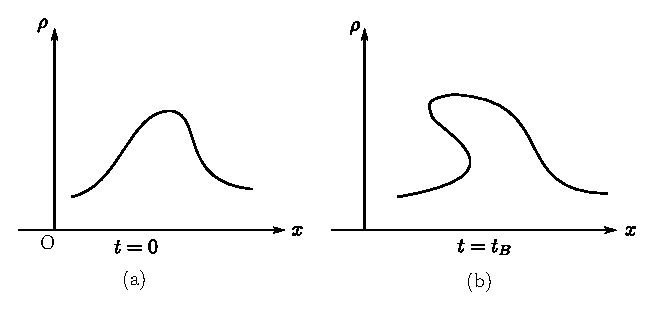
\includegraphics{figures/fig61-2.4.eps}
\caption{}
\label{chap1:fig2.4}
\end{figure}

Let $f$ be the initial distribution function as shown in the figure 2.4(a). Since $c'(\rho)=V'(\rho)<0$, breaking occurs on the left. The solution of the problem is 
\begin{align*}
\rho &= \rho(\xi)\\
x &= tF(\xi)+\xi\quad\text{where}\quad F(\xi)=c(f(\xi))
\end{align*}
Breaking occurs when $F'(\xi)<0$. But
$$
F'(\xi)=c'(f(\xi)). f'(\xi)<0\quad\text{iff}\quad f'(\xi)>0
$$
\ie when $f$ is increasing.

In most other examples $c'(\rho)>0$, so that a wave of increasing density breaks at the front.

\section{Flood waves in rivers}\pageoriginale\label{chap2:sec2.2}

Another example comes from an approximate theory for flood waves in rivers. For simplicity we take a rectangular channel of constant breadth, and assume that the disturbance is roughly the same across the breadth. Then the height $h(x,t)$ plays the role of `density'. Let $\rho$ be the flow per unit breadth, per unit time. Then from the conservation law we have 
$$
\frac{d}{dt}\int\limits_{x_2}^{x_1}h\,dx+q_1-q_2=0
$$
Taking the limit $x_2\to x_1$, we obtain
$$
h_t+q_x=0
$$
A functional relation $q=Q(h)$ is a good first approximation when the river is flooding. Therefore the governing equation is 
$$
h_t+c(h)h_x=0
$$
where $c(h)=\frac{dQ}{dh}$.

This formula for the wave speed was first proposed by Kleitz and Seddon. The function $Q(h)$ is determined from a balance between gravitational acceleration down the sloping bed and frictional effects. When the function is given by the Chezy formula $V\alpha h^{1/2}$ \ie $V=kh^{1/2}$, where $V$ is the velocity of the flow, we have
$$
Q(h)=Vh=kh^{3/2}
$$
and $c(h)=\frac{3}{2} kh^{1/2}=\frac{3}{2}V$. According\pageoriginale to this, flood waves move roughly half as fast again as the stream.

\section{Chemical exchange processes}\label{chap2:sec2.3}

In chemical engineering various processes concern a flow of fluid carrying some substances or particles through a solid bed. In the process some part of the material in the fluid will be deposited on the solid bed. In a simple formulation we assume that the fluid has constant velocity $V$. We take density to be $\rho=\rho_f+\rho_s$, where $\rho_f$ is the density of the substance concerned in the fluid and $\rho_s$ is the density of the material deposited on solid bed. The total flow of material across any section is 
$$
q=\rho_f V.
$$

The conservation equation becomes
\begin{equation}
\frac{\partial}{\partial t}\left(\rho_{_f} +
\rho_s\right)+V\frac{\partial\rho_f} {\partial x} =
0\tag{2.4}\label{chap2:eq2.4} 
\end{equation}
To complete the system we require more equations. When the changes are
slow we can assume to a first approximation that is a
quasi - equilibrium between the amounts in the fluid and on the solid
and that this balance leads to a functional relation
$\rho_s=R(\rho_f)$. Then \eqref{chap2:eq2.4} becomes 
\begin{gather*}
\frac{\partial}{\partial t}\rho_f +c(\rho_f)\frac{\partial}{\partial x}\rho_f=0\\
\intertext{where}
c(\rho_f)=\frac{V}{1+R'(\rho_f)}.
\end{gather*}

The\pageoriginale relation between $\rho_f$ and $\rho_s$ is discussed in more detail below (see 3.6).

\section{Glaciers}\label{chap2:sec2.4}

Nye (1960, 1963) has pointed out that the ideas on flood waves apply equally to the study of waves on glaciers and has developed the particular aspects that are most important there. He refers to Finsterwalder (1907) for the first studies of wave motion on glaciers and to independent formulations by Weertman (1958). For order of magnitude purposes, one may take
$$
Q(h)\propto h^N
$$
with $N$ roughly in the range 3 to 5. The propagation speed is 
$$
c=\frac{dQ}{dh}=Nv,
$$
where $v$ is the average velocity $Q/h$. Thus the waves move about three to five times faster than the average flow velocity. Typical velocities are of the order of 10 to 100 metres per year.

An interesting question considered by Nye is the effect of periodic accumulation and evaporation of the ice; depending on the period, this may refer either to seasonal or climatic changes. To do this, a prescribed source term $f(x,t)$ is added to the continuity equation; that is one takes
$$
h_t+q_x=f(x,t),q=Q(h,x).
$$

The consequences are determined from integration of the characteristic equations
\begin{align*}
\frac{dh}{dt} &= f(x,t)-Q_x(h,x),\\
\frac{dx}{dt} &= Q_h(h,x).
\end{align*}\pageoriginale

The main results in that parts of the glacier may be very sensitive, and relatively rapid local changes can be triggered by the source term.

\section{Erosion}\label{chap2:sec2.5}

Erosion in mountains was studied by Luke. Let $h(x,t)$ be the height of the mountain from the ground level. It is reasonable to assume a functional relation between $h_t$ and $h_x$ as:
$$
h_t=-Q\left(h_x\right).
$$
(When the slope of the mountain is greater, it is more vulnerable to erosion).

Let
\begin{equation}
s=h_x\tag{2.5}\label{chap2:eq2.5}
\end{equation}
Then differentiating \eqref{chap2:eq2.5} with respect to $x$ we obtain 
$$
h_{tx}=-Q'\left(h_x\right)h_{xx},
$$
that is $\dfrac{\partial s}{\partial t}+Q'(s)\dfrac{\partial
  s}{\partial x}=0$, which is our one dimensional non-linear wave
equation with $c(s)=Q'(s)$. When breaking occurs we introduce
discontinuities in $s$, which is $h_x$, and $h$ remains continuous but
with a sharp corner. 
